
\section{shelves and streams}


\subsection{shallow shelf aprx (SSA)}

\begin{frame}{flow model II: shallow shelf approximation stress balance (= SSA)}

SSA model applies very well to \alert{ice shelves}
\begin{itemize}
\item away from grounding lines
\item \dots and calving fronts
\end{itemize}

\bigskip\bigskip

\begin{center}
  \includegraphics[width=0.6\textwidth]{iceshelfedge}

\tiny edge of Ekstr\"om ice shelf (Hans Grobe)
\end{center}
\end{frame}


\begin{frame}{shallow shelf approximation stress balance 2}

SSA also applies reasonably well to \alert{ice streams}
\begin{itemize}
\item with modest bed topography
\item \dots and weak bed strength\footnote{energy conservation (esp.~basal melt rate) and subglacial hydrology (esp.~effective pressure) are major aspects of models of ice stream flow \dots \emph{not addressed here}}
\item imperfect near shear margins and grounding lines
\end{itemize}

\begin{center}
  \includegraphics[width=0.6\textwidth]{siple}

\tiny surface velocity for Siple Coast ice streams, Antarctica 
\end{center}
\end{frame}


\begin{frame}{what is, \emph{and is not}, an ice stream?}

\begin{columns}
\begin{column}{0.6\textwidth}
\begin{itemize}
\item ice streams
  \small
  \begin{itemize}
  \item[$\circ$] slide ($100$--$1000 \,\text{m}\,\text{a}^{-1}$)
  \item[$\circ$] have concentrated vertical shear in thin layer near base
  \end{itemize}
  \normalsize
\item ``outlet glaciers''
  \begin{itemize}
  \item[$\circ$] fast surface speed ($\sim10 \,\text{km}\,\text{a}^{-1}$)
    \begin{itemize}
    \item \dots not clear how much is sliding
    \end{itemize}    
  \item[$\circ$] substantial bed topography
  \item[$\circ$] thick layer of soft temperate ice
  \item[$\circ$] substantial vertical shear ``up'' in the ice column
  \end{itemize}
\item \alert{few simplifying assumptions are appropriate for outlet glaciers}
\end{itemize}
\end{column}

\begin{column}{0.4\textwidth}
\includegraphics[width=1.0\textwidth]{streamisbrae}

\bigskip
\scriptsize
Jakobshavns Isbrae (\textbf{a}) and Whillans Ice Stream (\textbf{b}); plotted without vertical exaggeration (\tiny Truffer and Echelmeyer (2003), \emph{Of isbrae and ice streams}\scriptsize)
\end{column}
\end{columns}
\end{frame}


\begin{frame}{SSA stress balance equation}

\begin{itemize}
\item only plane flow (``flow line'') case here
\item this equation determines velocity $u$ in an \emph{ice stream}:
\begin{empheq}[box=\fbox]{equation}
  \left({\color{red}2 A^{-1/n} H |u_x|^{1/n - 1} u_x}\right)_x - {\color{blue}C|u|^{m-1}u} = {\color{green}\rho g H h_x} \label{ssa}
\end{empheq}
\item the {\color{red} red term} inside parentheses is the vertically-integrated ``longitudinal'' or ``membrane'' stress
\item the {\color{blue} blue term} is basal resistance
  \begin{itemize}
  \item[$\circ$] this term is zero in an \emph{ice shelf}
  \end{itemize}
\item the {\color{green} green term} is  driving stress

\bigskip
\item \emph{how to think about this equation}?
\item \emph{how do you solve it numerically}?
\end{itemize}
\end{frame}


\begin{frame}{SSA context: from stream to shelf}

\begin{itemize}
\item here is what a 1D ``marine ice sheet model'' looks like:
\end{itemize}
\small
\begin{align*}
  u = u_0 & \qquad \text{ at } x = 0 \\
  \left.\begin{array}{r}
  \left(2 A^{-1/n} H |u_x|^{1/n - 1} u_x\right)_x - C|u|^{m-1}u = \rho g H h_x \\
  h = H + b
  \end{array}\right\}& \qquad \text{ on } 0 < x < x_g \\
  \left.\begin{array}{r}
  \left(2 A^{-1/n} H |u_x|^{1/n - 1} u_x\right)_x + 0 = \rho g H h_x \\
  h = (1-\rho/\rho_w) H
  \end{array}\right\}& \qquad \text{ on } x_g < x < x_c \\
  2 A^{-1/n} H |u_x|^{1/n - 1} u_x = \frac{1}{2}\rho (1-\rho/\rho_w) g H^2 & \qquad \text{ at } x = x_c
\end{align*}

\smallskip
\begin{center}
  \includegraphics[width=0.85\textwidth]{flowline}
\end{center}
\end{frame}


\begin{frame}{flotation criterion and grounding line}

\begin{itemize}
\item inequality ``$\rho H < - \rho_w b$'' for floating ice is the \alert{flotation criterion}
\item at the grounding line $x=x_g$ get equality: $\rho H = - \rho_w b$
\item the driving stress switches form at the grounding line:
  \begin{itemize}
  \item[$\circ$] on the grounded side:
    $$\rho g H h_x = \rho g H (H_x + b_x)$$
  \item[$\circ$] on the floating side, since Archimedes says $h = (1-\rho/\rho_w) H$:
    $$\rho g H h_x = \rho(1-\rho/\rho_w) g H H_x$$
  \end{itemize}
\end{itemize}
\end{frame}



\subsection{ice shelf flow line solution}


\begin{frame}{exact velocity and thickness for steady ice shelf}

\begin{itemize}
\item limited goal here: describe a steady state, 1D ice shelf
\item it is a nice \alert{by-hand} exact solution (next slide; see exercises) to both the stress balance and mass continuity equations
\item in 1D the thickness and velocity functions in the ice shelf are determined by just two numbers at grounding line $x_g=0$:
  \begin{itemize}
  \item[$\circ$] thickness $H_g$
  \item[$\circ$] velocity $u_g$
  \end{itemize}
\item we will use this to
  \begin{itemize}
  \item[$\circ$] understand the SSA better
  \item[$\circ$] verify a numerical SSA code
  \end{itemize}
\end{itemize}
\end{frame}


\begin{frame}{exact velocity and thickness for steady ice shelf \quad 2}

\small
\begin{itemize}
\item see \texttt{testshelf.m}
\item here $H_g=500$ m, $u_g=50$ m/a
\end{itemize}

\bigskip
\begin{columns}
  \begin{column}{0.5\textwidth}
  \includegraphics[width=1.0\textwidth]{steadyshelfprofile}
  
  \begin{center}  
  $h(x)$ and $b(x)$
  \end{center}
  \end{column}
  \begin{column}{0.5\textwidth}
  \includegraphics[width=1.0\textwidth]{steadyshelfvelocity}

  \begin{center}  
  velocity $u(x)$
  \end{center}
  \end{column}
\end{columns}

\bigskip
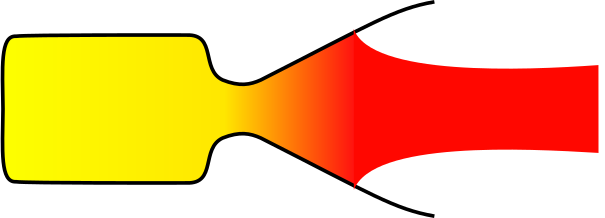
\includegraphics[width=0.25\textwidth]{Rocket_nozzle_expansion}
\end{frame}


\subsection{numerical SSA}

\begin{frame}{numerically solving the SSA stress balance}

\begin{itemize}
\item for an example, we fix ice thickness $H(x)$ and find the velocity numerically
\item recall the stress balance is a nonlinear equation for velocity:
  $$\left(2 A^{-1/n} H |u_x|^{1/n - 1} u_x\right)_x - C|u|^{m-1}u = \rho g H h_x$$
\item \alert{iteration is needed}
\item I'll describe the numerical method for a shelf \emph{or} stream, but only give a code for an ice shelf
\end{itemize}
\end{frame}


\begin{frame}{numerically solving the SSA stress balance 2}

\begin{itemize}
\item coefficient ${\color{red} \bar \nu} = A^{-1/n} |u_x|^{1/n-1}$ is the ``effective viscosity'':
   $$\left(2 \,{\color{red} \bar \nu}\, H u_x\right)_x - C |u|^{m-1} u = \rho g H h_x$$

\medskip
\item \emph{simplest iteration idea}: use old effective viscosity to get new velocity solution, and repeat until things stop changing
  \begin{itemize}
  \item[$\circ$] this is ``Picard'' iteration
  \item[$\circ$] Newton iteration is a superior alternative
  \end{itemize}

\bigskip
\item recipe starts with initial iterate $u^{(0)}$, then:
  \begin{itemize}
  \item[$\circ$] define $\bar \nu^{(k-1)} = A^{-1/n} |u^{(k-1)}_x|^{1/n-1}$ from last iterate $u^{(k-1)}$
  \item[$\circ$] current iterate (unknown) $u^{(k)}$
  \item[$\circ$] solve repeatedly:
     $$\left(2 \bar \nu^{(k-1)} H u^{(k)}_x\right)_x - C |u^{(k-1)}|^{m-1} u^{(k)} = \rho g H h_x$$
  \end{itemize}
\end{itemize}
\end{frame}


\begin{frame}{solving the ``inner'' linear problem}
\begin{itemize}
\item abstract the problem:
   $$\left(W(x)\, u_x\right)_x - \alpha(x)\, u = \beta(x)$$
on $0 < x < L$, with boundary conditions
   $$u(0) = V, \qquad  u_x(L) = \gamma$$
\item an \emph{elliptic} PDE boundary value problem
\item $W(x)$, $\alpha(x)$, $\beta(x)$ are known functions in the SSA context:
  \begin{itemize}
  \item[$\circ$] both $W(x)$ and $\alpha(x)$ come from previous iteration
  \item[$\circ$] $\beta(x)$ is driving stress
  \end{itemize}
\end{itemize}
\end{frame}


\begin{frame}{where do you get an initial guess $u^{(0)}$?}

\begin{itemize}
\item \emph{for floating ice}, use velocity from assuming a uniform strain rate:
   $$u^{(0)}(x) = \gamma (x-x_g) + u_g$$
where $\gamma$ is the value of $u_x$ found from calving front stress imbalance
\item \emph{for grounded ice}, use velocity from assuming ice is held by basal resistance only:
   $$u^{(0)}(x) = \left(-C^{-1} \rho g H h_x\right)^{1/m}$$
\end{itemize}
\end{frame}


\begin{frame}{numerics of the ``inner'' linear problem}

\begin{itemize}
\item index $j=1,2,\dots,J+1$
\item $x_1 = x_g$ and $x_{J+1} = x_c$ are endpoints
\item $W(x)$ is needed on the staggered grid; the approximation is:
$$\frac{W_{j+1/2} (u_{j+1} - u_j) - W_{j-1/2} (u_{j} - u_{j-1})}{\Delta x^2} - \alpha_j u_j \stackrel{\ast}{=} \beta_j$$
\item left-hand boundary condition: $u_1 = V$ given
\item right-hand boundary condition (``$u_x(L)=\gamma$''):
  \begin{itemize}
  \item[$\circ$] introduce notional point $x_{J+2}$ and use equation
    $$\frac{u_{J+2} - u_J}{2 \Delta x} = \gamma$$
  \item[$\circ$] using equation $\ast$ in $j=J+1$ case, eliminate $u_{J+2}$ variable ``by-hand'' before coding numerics
  \end{itemize}
\end{itemize}
\end{frame}


\begin{frame}{numerics of the ``inner'' linear problem 2}

\begin{itemize}
\small
\item so SSA stress balance has form  \quad $A \mathbf{x} = \mathbf{b}$, \quad namely:
\scriptsize
$$
\begin{bmatrix}
1 &  &  &  &  \\
W_{3/2} & A_{22} & W_{5/2} &  &  \\
 & W_{5/2} & A_{33} &  &  \\
 &  & \ddots & \ddots &  \\
 &  & W_{J-1/2} & A_{JJ} & W_{J+1/2} \\
 &  &  & A_{J+1,J} & A_{J+1,J+1} \\
\end{bmatrix}\,
\begin{bmatrix}
u_1 \\ u_2 \\ u_3 \\ \vdots \\ u_J \\ u_{J+1}
\end{bmatrix}
=
\begin{bmatrix}
0 \\ \beta_2 \Delta x^2 \\ \beta_3 \Delta x^2 \\ \vdots \\ \beta_J \Delta x^2 \\ b_{J+1}
\end{bmatrix}
$$
with diagonal entries
$$A_{22} = -(W_{3/2}+W_{5/2}+\alpha_1 \Delta x^2)$$
$$A_{33} = -(W_{5/2}+W_{7/2}+\alpha_2 \Delta x^2)$$
and so on, up to $A_{JJ}$, and with special cases in last equation:
$$A_{J+1,J} = 2 W_{J+1/2}$$
$$A_{J+1,J+1} = -(2 W_{J+1/2}+\alpha_{J+1}\Delta x^2)$$
$$b_{J+1} = -2 \gamma \Delta x W_{J+3/2} + \beta_{J+1} \Delta x^2$$

\small
\smallskip
\item this is a \emph{tridiagonal} linear system
\item give it to a matrix-solving black box!
\end{itemize}
\end{frame}


\begin{frame}{numerics of the ``inner'' linear problem 3}

\minput{flowline}

\vspace{-5mm}
\begin{itemize}
\item solves
  $$\left(W(x)u_x\right)_x - \alpha(x) u = \beta(x)$$
\end{itemize}
\end{frame}


\begin{frame}{testing the ``inner'' linear code}

\begin{itemize}
\item before proceeding to solve nonlinear SSA problem, we can test the ``abstracted'' code \texttt{flowline.m}
\item test by ``manufacturing'' solutions
  \begin{itemize}
  \item[$\circ$] see \texttt{testflowline.m}; not shown
  \end{itemize}
\item results:
  \begin{itemize}
  \item[$\circ$] converges at optimal rate $O(\Delta x^2)$
  \end{itemize}
\end{itemize}
\end{frame}


\begin{frame}{numerical SSA}

\minputtiny{ssaflowline}

\vspace{-3mm}
\small
\begin{itemize}
\item solves
  $$\left(2 A^{-1/n} H |u_x|^{1/n - 1} u_x\right)_x - C|u|^{m-1}u = \rho g H h_x$$
\end{itemize}
\end{frame}


\begin{frame}{numerical SSA model results}

\begin{itemize}
\item \texttt{testshelf.m} (not shown) applies \texttt{ssaflowline.m} with same boundary conditions as exact solution; get
\end{itemize}

\begin{center}
  \includegraphics[width=0.45\textwidth]{steadyshelfprofile} \quad
  \includegraphics[width=0.45\textwidth]{steadyshelfvelocity}
\end{center}

\bigskip
\begin{itemize}
\item \emph{this looks suspiciously like figures for the exact solution \dots}
\item yes
\end{itemize}
\end{frame}


\begin{frame}{\emph{numerical} thickness and velocity for steady ice shelf}

\begin{itemize}
\item ``convergence analysis'' means looking at exact/numerical difference as grid is refined
\item below: convergence analysis of velocity from \texttt{testshelf.m}
\end{itemize}

\begin{center}
  \includegraphics[width=0.7\textwidth]{shelfconv}
\end{center}
\end{frame}


\begin{frame}{realistic ice shelf modeling}

\begin{itemize}
\item flow lines are never very realistic
\item real ice shelves have ``side drag''
  \begin{itemize}
  \item[$\circ$] one can parameterize it \dots
  \end{itemize}
\item real ice shelves have more processes:
  \begin{itemize}
  \item[$\circ$] high basal melt near grounding lines
  \item[$\circ$] marine ice freeze-on at bottom (below)
  \item[$\circ$] fractures and calving
  \end{itemize}
\item real ice shelves have nontrivial dynamics:
  \begin{itemize}
  \item[$\circ$] ``reverse slope'' bed instability and WAIS \dots
  \end{itemize}
\end{itemize}

\medskip
\begin{center}
  \includegraphics[width=0.5\textwidth]{marineice}
  
  \medskip
  \tiny from Grosfeld \& Thyssen 1994
\end{center}
\end{frame}


\begin{frame}{ice shelf modeling in 2D}

\begin{itemize}
\item nonetheless ``diagnostic'' (static geometry) ice shelf modeling in 2D has been quite successful
\item observed surface velocities validate SSA model
  \begin{itemize}
  \item[$\circ$] e.g.~Ross ice shelf example below using PISM
  \item[$\circ$] \dots but many models can do this
  \end{itemize}
\end{itemize}

\begin{center}
  \includegraphics[width=0.5\textwidth]{rossquiver} \quad  \includegraphics[width=0.45\textwidth]{rossscatter}
\end{center}
\end{frame}
